\documentclass[1p]{elsarticle_modified}
%\bibliographystyle{elsarticle-num}

%\usepackage[colorlinks]{hyperref}
%\usepackage{abbrmath_seonhwa} %\Abb, \Ascr, \Acal ,\Abf, \Afrak
\usepackage{amsfonts}
\usepackage{amssymb}
\usepackage{amsmath}
\usepackage{amsthm}
\usepackage{scalefnt}
\usepackage{amsbsy}
\usepackage{kotex}
\usepackage{caption}
\usepackage{subfig}
\usepackage{color}
\usepackage{graphicx}
\usepackage{xcolor} %% white, black, red, green, blue, cyan, magenta, yellow
\usepackage{float}
\usepackage{setspace}
\usepackage{hyperref}

\usepackage{tikz}
\usetikzlibrary{arrows}

\usepackage{multirow}
\usepackage{array} % fixed length table
\usepackage{hhline}

%%%%%%%%%%%%%%%%%%%%%
\makeatletter
\renewcommand*\env@matrix[1][\arraystretch]{%
	\edef\arraystretch{#1}%
	\hskip -\arraycolsep
	\let\@ifnextchar\new@ifnextchar
	\array{*\c@MaxMatrixCols c}}
\makeatother %https://tex.stackexchange.com/questions/14071/how-can-i-increase-the-line-spacing-in-a-matrix
%%%%%%%%%%%%%%%

\usepackage[normalem]{ulem}

\newcommand{\msout}[1]{\ifmmode\text{\sout{\ensuremath{#1}}}\else\sout{#1}\fi}
%SOURCE: \msout is \stkout macro in https://tex.stackexchange.com/questions/20609/strikeout-in-math-mode

\newcommand{\cancel}[1]{
	\ifmmode
	{\color{red}\msout{#1}}
	\else
	{\color{red}\sout{#1}}
	\fi
}

\newcommand{\add}[1]{
	{\color{blue}\uwave{#1}}
}

\newcommand{\replace}[2]{
	\ifmmode
	{\color{red}\msout{#1}}{\color{blue}\uwave{#2}}
	\else
	{\color{red}\sout{#1}}{\color{blue}\uwave{#2}}
	\fi
}

\newcommand{\Sol}{\mathcal{S}} %segment
\newcommand{\D}{D} %diagram
\newcommand{\A}{\mathcal{A}} %arc


%%%%%%%%%%%%%%%%%%%%%%%%%%%%%5 test

\def\sl{\operatorname{\textup{SL}}(2,\Cbb)}
\def\psl{\operatorname{\textup{PSL}}(2,\Cbb)}
\def\quan{\mkern 1mu \triangleright \mkern 1mu}

\theoremstyle{definition}
\newtheorem{thm}{Theorem}[section]
\newtheorem{prop}[thm]{Proposition}
\newtheorem{lem}[thm]{Lemma}
\newtheorem{ques}[thm]{Question}
\newtheorem{cor}[thm]{Corollary}
\newtheorem{defn}[thm]{Definition}
\newtheorem{exam}[thm]{Example}
\newtheorem{rmk}[thm]{Remark}
\newtheorem{alg}[thm]{Algorithm}

\newcommand{\I}{\sqrt{-1}}
\begin{document}

%\begin{frontmatter}
%
%\title{Boundary parabolic representations of knots up to 8 crossings}
%
%%% Group authors per affiliation:
%\author{Yunhi Cho} 
%\address{Department of Mathematics, University of Seoul, Seoul, Korea}
%\ead{yhcho@uos.ac.kr}
%
%
%\author{Seonhwa Kim} %\fnref{s_kim}}
%\address{Center for Geometry and Physics, Institute for Basic Science, Pohang, 37673, Korea}
%\ead{ryeona17@ibs.re.kr}
%
%\author{Hyuk Kim}
%\address{Department of Mathematical Sciences, Seoul National University, Seoul 08826, Korea}
%\ead{hyukkim@snu.ac.kr}
%
%\author{Seokbeom Yoon}
%\address{Department of Mathematical Sciences, Seoul National University, Seoul, 08826,  Korea}
%\ead{sbyoon15@snu.ac.kr}
%
%\begin{abstract}
%We find all boundary parabolic representation of knots up to 8 crossings.
%
%\end{abstract}
%\begin{keyword}
%    \MSC[2010] 57M25 
%\end{keyword}
%
%\end{frontmatter}

%\linenumbers
%\tableofcontents
%
\newcommand\colored[1]{\textcolor{white}{\rule[-0.35ex]{0.8em}{1.4ex}}\kern-0.8em\color{red} #1}%
%\newcommand\colored[1]{\textcolor{white}{ #1}\kern-2.17ex	\textcolor{white}{ #1}\kern-1.81ex	\textcolor{white}{ #1}\kern-2.15ex\color{red}#1	}

{\Large $\underline{12n_{0770}~(K12n_{0770})}$}

\setlength{\tabcolsep}{10pt}
\renewcommand{\arraystretch}{1.6}
\vspace{1cm}\begin{tabular}{m{100pt}>{\centering\arraybackslash}m{274pt}}
\multirow{5}{120pt}{
	\centering
	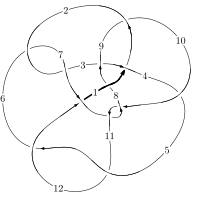
\includegraphics[width=112pt]{../../../GIT/diagram.site/Diagrams/png/2859_12n_0770.png}\\
\ \ \ A knot diagram\footnotemark}&
\allowdisplaybreaks
\textbf{Linearized knot diagam} \\
\cline{2-2}
 &
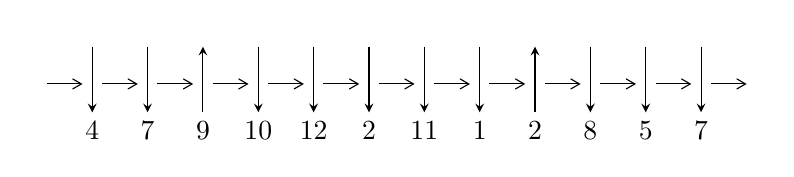
\begin{tikzpicture}[x=20pt, y=17pt]
	% nodes
	\node (C0) at (0, 0) {};
	\node (C1) at (1, 0) {};
	\node (C1U) at (1, +1) {};
	\node (C1D) at (1, -1) {4};

	\node (C2) at (2, 0) {};
	\node (C2U) at (2, +1) {};
	\node (C2D) at (2, -1) {7};

	\node (C3) at (3, 0) {};
	\node (C3U) at (3, +1) {};
	\node (C3D) at (3, -1) {9};

	\node (C4) at (4, 0) {};
	\node (C4U) at (4, +1) {};
	\node (C4D) at (4, -1) {10};

	\node (C5) at (5, 0) {};
	\node (C5U) at (5, +1) {};
	\node (C5D) at (5, -1) {12};

	\node (C6) at (6, 0) {};
	\node (C6U) at (6, +1) {};
	\node (C6D) at (6, -1) {2};

	\node (C7) at (7, 0) {};
	\node (C7U) at (7, +1) {};
	\node (C7D) at (7, -1) {11};

	\node (C8) at (8, 0) {};
	\node (C8U) at (8, +1) {};
	\node (C8D) at (8, -1) {1};

	\node (C9) at (9, 0) {};
	\node (C9U) at (9, +1) {};
	\node (C9D) at (9, -1) {2};

	\node (C10) at (10, 0) {};
	\node (C10U) at (10, +1) {};
	\node (C10D) at (10, -1) {8};

	\node (C11) at (11, 0) {};
	\node (C11U) at (11, +1) {};
	\node (C11D) at (11, -1) {5};

	\node (C12) at (12, 0) {};
	\node (C12U) at (12, +1) {};
	\node (C12D) at (12, -1) {7};
	\node (C13) at (13, 0) {};

	% arrows
	\draw[->,>={angle 60}]
	(C0) edge (C1) (C1) edge (C2) (C2) edge (C3) (C3) edge (C4) (C4) edge (C5) (C5) edge (C6) (C6) edge (C7) (C7) edge (C8) (C8) edge (C9) (C9) edge (C10) (C10) edge (C11) (C11) edge (C12) (C12) edge (C13) ;	\draw[->,>=stealth]
	(C1U) edge (C1D) (C2U) edge (C2D) (C3D) edge (C3U) (C4U) edge (C4D) (C5U) edge (C5D) (C6U) edge (C6D) (C7U) edge (C7D) (C8U) edge (C8D) (C9D) edge (C9U) (C10U) edge (C10D) (C11U) edge (C11D) (C12U) edge (C12D) ;
	\end{tikzpicture} \\
\hhline{~~} \\& 
\textbf{Solving Sequence} \\ \cline{2-2} 
 &
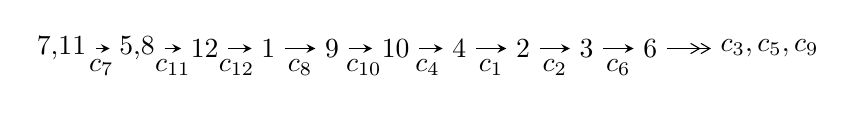
\begin{tikzpicture}[x=23pt, y=7pt]
	% node
	\node (A0) at (-1/8, 0) {7,11};
	\node (A1) at (17/16, 0) {5,8};
	\node (A2) at (17/8, 0) {12};
	\node (A3) at (25/8, 0) {1};
	\node (A4) at (33/8, 0) {9};
	\node (A5) at (41/8, 0) {10};
	\node (A6) at (49/8, 0) {4};
	\node (A7) at (57/8, 0) {2};
	\node (A8) at (65/8, 0) {3};
	\node (A9) at (73/8, 0) {6};
	\node (C1) at (1/2, -1) {$c_{7}$};
	\node (C2) at (13/8, -1) {$c_{11}$};
	\node (C3) at (21/8, -1) {$c_{12}$};
	\node (C4) at (29/8, -1) {$c_{8}$};
	\node (C5) at (37/8, -1) {$c_{10}$};
	\node (C6) at (45/8, -1) {$c_{4}$};
	\node (C7) at (53/8, -1) {$c_{1}$};
	\node (C8) at (61/8, -1) {$c_{2}$};
	\node (C9) at (69/8, -1) {$c_{6}$};
	\node (A10) at (11, 0) {$c_{3},c_{5},c_{9}$};

	% edge
	\draw[->,>=stealth]	
	(A0) edge (A1) (A1) edge (A2) (A2) edge (A3) (A3) edge (A4) (A4) edge (A5) (A5) edge (A6) (A6) edge (A7) (A7) edge (A8) (A8) edge (A9) ;
	\draw[->>,>={angle 60}]	
	(A9) edge (A10);
\end{tikzpicture} \\ 

\end{tabular} \\

\footnotetext{
The image of knot diagram is generated by the software ``\textbf{Draw programme}" developed by Andrew Bartholomew(\url{http://www.layer8.co.uk/maths/draw/index.htm\#Running-draw}), where we modified some parts for our purpose(\url{https://github.com/CATsTAILs/LinksPainter}).
}\phantom \\ \newline 
\centering \textbf{Ideals for irreducible components\footnotemark of $X_{\text{par}}$} 
 
\begin{align*}
I^u_{1}&=\langle 
1.64367\times10^{347} u^{113}-1.16814\times10^{348} u^{112}+\cdots+8.26301\times10^{347} b-1.41159\times10^{349},\\
\phantom{I^u_{1}}&\phantom{= \langle  }-1.42691\times10^{349} u^{113}+8.15610\times10^{349} u^{112}+\cdots+3.47046\times10^{349} a+1.77529\times10^{350},\\
\phantom{I^u_{1}}&\phantom{= \langle  }u^{114}-5 u^{113}+\cdots-28 u+28\rangle \\
I^u_{2}&=\langle 
7.56683\times10^{20} u^{38}-7.68268\times10^{21} u^{37}+\cdots+1.46846\times10^{20} b-2.75750\times10^{21},\\
\phantom{I^u_{2}}&\phantom{= \langle  }-1.42755\times10^{20} u^{38}+2.29096\times10^{21} u^{37}+\cdots+5.87384\times10^{20} a-8.95365\times10^{21},\\
\phantom{I^u_{2}}&\phantom{= \langle  }u^{39}-11 u^{38}+\cdots+44 u-4\rangle \\
I^u_{3}&=\langle 
b+1,\;a+1,\;u-1\rangle \\
\\
\end{align*}
\raggedright * 3 irreducible components of $\dim_{\mathbb{C}}=0$, with total 154 representations.\\
\footnotetext{All coefficients of polynomials are rational numbers. But the coefficients are sometimes approximated in decimal forms when there is not enough margin.}
\newpage
\renewcommand{\arraystretch}{1}
\centering \section*{I. $I^u_{1}= \langle 1.64\times10^{347} u^{113}-1.17\times10^{348} u^{112}+\cdots+8.26\times10^{347} b-1.41\times10^{349},\;-1.43\times10^{349} u^{113}+8.16\times10^{349} u^{112}+\cdots+3.47\times10^{349} a+1.78\times10^{350},\;u^{114}-5 u^{113}+\cdots-28 u+28 \rangle$}
\flushleft \textbf{(i) Arc colorings}\\
\begin{tabular}{m{7pt} m{180pt} m{7pt} m{180pt} }
\flushright $a_{7}=$&$\begin{pmatrix}1\\0\end{pmatrix}$ \\
\flushright $a_{11}=$&$\begin{pmatrix}0\\u\end{pmatrix}$ \\
\flushright $a_{5}=$&$\begin{pmatrix}0.411157 u^{113}-2.35015 u^{112}+\cdots+37.1094 u-5.11544\\-0.198919 u^{113}+1.41370 u^{112}+\cdots-38.8486 u+17.0833\end{pmatrix}$ \\
\flushright $a_{8}=$&$\begin{pmatrix}1\\u^2\end{pmatrix}$ \\
\flushright $a_{12}=$&$\begin{pmatrix}-0.250042 u^{113}+1.26176 u^{112}+\cdots-13.9324 u-0.971506\\-0.0132989 u^{113}-0.184376 u^{112}+\cdots+31.7660 u-17.9686\end{pmatrix}$ \\
\flushright $a_{1}=$&$\begin{pmatrix}-0.236744 u^{113}+1.44614 u^{112}+\cdots-45.6984 u+16.9971\\-0.0132989 u^{113}-0.184376 u^{112}+\cdots+31.7660 u-17.9686\end{pmatrix}$ \\
\flushright $a_{9}=$&$\begin{pmatrix}-0.801265 u^{113}+3.88615 u^{112}+\cdots-9.13740 u-25.0527\\0.354616 u^{113}-1.85556 u^{112}+\cdots+11.0496 u+4.41535\end{pmatrix}$ \\
\flushright $a_{10}=$&$\begin{pmatrix}u\\u^3+u\end{pmatrix}$ \\
\flushright $a_{4}=$&$\begin{pmatrix}0.488225 u^{113}-3.03280 u^{112}+\cdots+66.2774 u-19.6772\\-0.0385091 u^{113}+0.428468 u^{112}+\cdots-20.1635 u+10.8463\end{pmatrix}$ \\
\flushright $a_{2}=$&$\begin{pmatrix}-0.734453 u^{113}+3.50787 u^{112}+\cdots+0.813004 u-21.0445\\0.102327 u^{113}-0.625191 u^{112}+\cdots+8.52878 u-1.63632\end{pmatrix}$ \\
\flushright $a_{3}=$&$\begin{pmatrix}-0.836779 u^{113}+4.13306 u^{112}+\cdots-7.71577 u-19.4082\\0.102327 u^{113}-0.625191 u^{112}+\cdots+8.52878 u-1.63632\end{pmatrix}$ \\
\flushright $a_{6}=$&$\begin{pmatrix}-0.407728 u^{113}+2.54127 u^{112}+\cdots-50.8668 u+20.6255\\-0.136278 u^{113}+0.563144 u^{112}+\cdots+12.2868 u-8.91297\end{pmatrix}$\\&\end{tabular}
\flushleft \textbf{(ii) Obstruction class $= -1$}\\~\\
\flushleft \textbf{(iii) Cusp Shapes $= 1.09243 u^{113}-4.66473 u^{112}+\cdots-40.0688 u+38.8157$}\\~\\
\newpage\renewcommand{\arraystretch}{1}
\flushleft \textbf{(iv) u-Polynomials at the component}\newline \\
\begin{tabular}{m{50pt}|m{274pt}}
Crossings & \hspace{64pt}u-Polynomials at each crossing \\
\hline $$\begin{aligned}c_{1}\end{aligned}$$&$\begin{aligned}
&u^{114}-7 u^{113}+\cdots-6 u+1
\end{aligned}$\\
\hline $$\begin{aligned}c_{2},c_{6}\end{aligned}$$&$\begin{aligned}
&u^{114}+2 u^{113}+\cdots+40 u+1
\end{aligned}$\\
\hline $$\begin{aligned}c_{3}\end{aligned}$$&$\begin{aligned}
&u^{114}- u^{113}+\cdots+2622 u-51
\end{aligned}$\\
\hline $$\begin{aligned}c_{4}\end{aligned}$$&$\begin{aligned}
&u^{114}+2 u^{113}+\cdots+36042 u-2819
\end{aligned}$\\
\hline $$\begin{aligned}c_{5},c_{11}\end{aligned}$$&$\begin{aligned}
&u^{114}-29 u^{112}+\cdots-86783 u-21161
\end{aligned}$\\
\hline $$\begin{aligned}c_{7},c_{10}\end{aligned}$$&$\begin{aligned}
&u^{114}+5 u^{113}+\cdots+28 u+28
\end{aligned}$\\
\hline $$\begin{aligned}c_{8}\end{aligned}$$&$\begin{aligned}
&u^{114}-3 u^{113}+\cdots-18432 u-4096
\end{aligned}$\\
\hline $$\begin{aligned}c_{9}\end{aligned}$$&$\begin{aligned}
&u^{114}-3 u^{112}+\cdots-2209436 u-262349
\end{aligned}$\\
\hline $$\begin{aligned}c_{12}\end{aligned}$$&$\begin{aligned}
&u^{114}+8 u^{113}+\cdots+711116424 u-32039577
\end{aligned}$\\
\hline
\end{tabular}\\~\\
\newpage\renewcommand{\arraystretch}{1}
\flushleft \textbf{(v) Riley Polynomials at the component}\newline \\
\begin{tabular}{m{50pt}|m{274pt}}
Crossings & \hspace{64pt}Riley Polynomials at each crossing \\
\hline $$\begin{aligned}c_{1}\end{aligned}$$&$\begin{aligned}
&y^{114}-21 y^{113}+\cdots-24 y+1
\end{aligned}$\\
\hline $$\begin{aligned}c_{2},c_{6}\end{aligned}$$&$\begin{aligned}
&y^{114}+80 y^{113}+\cdots-214 y+1
\end{aligned}$\\
\hline $$\begin{aligned}c_{3}\end{aligned}$$&$\begin{aligned}
&y^{114}-15 y^{113}+\cdots+13651086 y+2601
\end{aligned}$\\
\hline $$\begin{aligned}c_{4}\end{aligned}$$&$\begin{aligned}
&y^{114}+10 y^{113}+\cdots-1131278350 y+7946761
\end{aligned}$\\
\hline $$\begin{aligned}c_{5},c_{11}\end{aligned}$$&$\begin{aligned}
&y^{114}-58 y^{113}+\cdots-10990689369 y+447787921
\end{aligned}$\\
\hline $$\begin{aligned}c_{7},c_{10}\end{aligned}$$&$\begin{aligned}
&y^{114}+65 y^{113}+\cdots-3920 y+784
\end{aligned}$\\
\hline $$\begin{aligned}c_{8}\end{aligned}$$&$\begin{aligned}
&y^{114}+25 y^{113}+\cdots+1644167168 y+16777216
\end{aligned}$\\
\hline $$\begin{aligned}c_{9}\end{aligned}$$&$\begin{aligned}
&y^{114}-6 y^{113}+\cdots-470658669282 y+68826997801
\end{aligned}$\\
\hline $$\begin{aligned}c_{12}\end{aligned}$$&$\begin{aligned}
&y^{114}+16 y^{113}+\cdots+5314413482865162 y+1026534494338929
\end{aligned}$\\
\hline
\end{tabular}\\~\\
\newpage\flushleft \textbf{(vi) Complex Volumes and Cusp Shapes}
$$\begin{array}{c|c|c}  
\text{Solutions to }I^u_{1}& \I (\text{vol} + \sqrt{-1}CS) & \text{Cusp shape}\\
 \hline 
\begin{aligned}
u &= \phantom{-}0.818099 + 0.532162 I \\
a &= \phantom{-}0.472412 - 1.199790 I \\
b &= \phantom{-}0.422644 + 0.059689 I\end{aligned}
 & \phantom{-}0.328422 + 0.462677 I & \phantom{-0.000000 } 0 \\ \hline\begin{aligned}
u &= \phantom{-}0.818099 - 0.532162 I \\
a &= \phantom{-}0.472412 + 1.199790 I \\
b &= \phantom{-}0.422644 - 0.059689 I\end{aligned}
 & \phantom{-}0.328422 - 0.462677 I & \phantom{-0.000000 } 0 \\ \hline\begin{aligned}
u &= -0.449141 + 0.924619 I \\
a &= \phantom{-}0.722724 + 0.463209 I \\
b &= \phantom{-}1.132120 + 0.424803 I\end{aligned}
 & -3.29175 - 0.83027 I & \phantom{-0.000000 } 0 \\ \hline\begin{aligned}
u &= -0.449141 - 0.924619 I \\
a &= \phantom{-}0.722724 - 0.463209 I \\
b &= \phantom{-}1.132120 - 0.424803 I\end{aligned}
 & -3.29175 + 0.83027 I & \phantom{-0.000000 } 0 \\ \hline\begin{aligned}
u &= \phantom{-}0.728416 + 0.601252 I \\
a &= -1.130000 + 0.764887 I \\
b &= -1.62485 - 0.52082 I\end{aligned}
 & -4.99624 - 2.74266 I & \phantom{-0.000000 } 0 \\ \hline\begin{aligned}
u &= \phantom{-}0.728416 - 0.601252 I \\
a &= -1.130000 - 0.764887 I \\
b &= -1.62485 + 0.52082 I\end{aligned}
 & -4.99624 + 2.74266 I & \phantom{-0.000000 } 0 \\ \hline\begin{aligned}
u &= \phantom{-}0.655193 + 0.841159 I \\
a &= \phantom{-}1.193410 - 0.082262 I \\
b &= \phantom{-}1.46588 + 0.07377 I\end{aligned}
 & \phantom{-}1.16863 - 5.87092 I & \phantom{-0.000000 } 0 \\ \hline\begin{aligned}
u &= \phantom{-}0.655193 - 0.841159 I \\
a &= \phantom{-}1.193410 + 0.082262 I \\
b &= \phantom{-}1.46588 - 0.07377 I\end{aligned}
 & \phantom{-}1.16863 + 5.87092 I & \phantom{-0.000000 } 0 \\ \hline\begin{aligned}
u &= \phantom{-}0.230146 + 1.049920 I \\
a &= -1.21464 - 0.94528 I \\
b &= -0.1186690 + 0.0768415 I\end{aligned}
 & \phantom{-}6.51073 + 0.29692 I & \phantom{-0.000000 } 0 \\ \hline\begin{aligned}
u &= \phantom{-}0.230146 - 1.049920 I \\
a &= -1.21464 + 0.94528 I \\
b &= -0.1186690 - 0.0768415 I\end{aligned}
 & \phantom{-}6.51073 - 0.29692 I & \phantom{-0.000000 } 0\\
 \hline 
 \end{array}$$\newpage$$\begin{array}{c|c|c}  
\text{Solutions to }I^u_{1}& \I (\text{vol} + \sqrt{-1}CS) & \text{Cusp shape}\\
 \hline 
\begin{aligned}
u &= -0.317192 + 1.028380 I \\
a &= -0.567236 - 1.102330 I \\
b &= -2.79481 - 0.02014 I\end{aligned}
 & \phantom{-}0.40066 + 5.93647 I & \phantom{-0.000000 } 0 \\ \hline\begin{aligned}
u &= -0.317192 - 1.028380 I \\
a &= -0.567236 + 1.102330 I \\
b &= -2.79481 + 0.02014 I\end{aligned}
 & \phantom{-}0.40066 - 5.93647 I & \phantom{-0.000000 } 0 \\ \hline\begin{aligned}
u &= -0.398064 + 0.830871 I \\
a &= \phantom{-}0.84701 + 1.59525 I \\
b &= \phantom{-}1.98160 - 0.64550 I\end{aligned}
 & -8.67291 + 1.70726 I & \phantom{-0.000000 } 0 \\ \hline\begin{aligned}
u &= -0.398064 - 0.830871 I \\
a &= \phantom{-}0.84701 - 1.59525 I \\
b &= \phantom{-}1.98160 + 0.64550 I\end{aligned}
 & -8.67291 - 1.70726 I & \phantom{-0.000000 } 0 \\ \hline\begin{aligned}
u &= \phantom{-}1.070220 + 0.165485 I \\
a &= \phantom{-}0.699806 - 0.687492 I \\
b &= \phantom{-}1.278800 + 0.301934 I\end{aligned}
 & -0.84358 + 2.42749 I & \phantom{-0.000000 } 0 \\ \hline\begin{aligned}
u &= \phantom{-}1.070220 - 0.165485 I \\
a &= \phantom{-}0.699806 + 0.687492 I \\
b &= \phantom{-}1.278800 - 0.301934 I\end{aligned}
 & -0.84358 - 2.42749 I & \phantom{-0.000000 } 0 \\ \hline\begin{aligned}
u &= -0.497495 + 0.768200 I \\
a &= -1.18960 - 1.20996 I \\
b &= -1.43561 - 0.00653 I\end{aligned}
 & -1.56140 - 1.49501 I & \phantom{-0.000000 } 0 \\ \hline\begin{aligned}
u &= -0.497495 - 0.768200 I \\
a &= -1.18960 + 1.20996 I \\
b &= -1.43561 + 0.00653 I\end{aligned}
 & -1.56140 + 1.49501 I & \phantom{-0.000000 } 0 \\ \hline\begin{aligned}
u &= -0.411146 + 0.795027 I \\
a &= -0.94055 - 1.73146 I \\
b &= -1.033310 + 0.482510 I\end{aligned}
 & -1.54985 + 5.31929 I & \phantom{-0.000000 } 0 \\ \hline\begin{aligned}
u &= -0.411146 - 0.795027 I \\
a &= -0.94055 + 1.73146 I \\
b &= -1.033310 - 0.482510 I\end{aligned}
 & -1.54985 - 5.31929 I & \phantom{-0.000000 } 0\\
 \hline 
 \end{array}$$\newpage$$\begin{array}{c|c|c}  
\text{Solutions to }I^u_{1}& \I (\text{vol} + \sqrt{-1}CS) & \text{Cusp shape}\\
 \hline 
\begin{aligned}
u &= \phantom{-}0.613156 + 0.940244 I \\
a &= -0.390137 + 0.753374 I \\
b &= -0.71225 - 1.22658 I\end{aligned}
 & -1.73750 - 3.98044 I & \phantom{-0.000000 } 0 \\ \hline\begin{aligned}
u &= \phantom{-}0.613156 - 0.940244 I \\
a &= -0.390137 - 0.753374 I \\
b &= -0.71225 + 1.22658 I\end{aligned}
 & -1.73750 + 3.98044 I & \phantom{-0.000000 } 0 \\ \hline\begin{aligned}
u &= -1.015600 + 0.496700 I \\
a &= -0.524971 - 0.785875 I \\
b &= -1.381690 + 0.126492 I\end{aligned}
 & -2.38932 - 4.78544 I & \phantom{-0.000000 } 0 \\ \hline\begin{aligned}
u &= -1.015600 - 0.496700 I \\
a &= -0.524971 + 0.785875 I \\
b &= -1.381690 - 0.126492 I\end{aligned}
 & -2.38932 + 4.78544 I & \phantom{-0.000000 } 0 \\ \hline\begin{aligned}
u &= -0.509445 + 1.019500 I \\
a &= \phantom{-}0.930280 + 0.220948 I \\
b &= \phantom{-}1.44465 - 1.35754 I\end{aligned}
 & \phantom{-}6.81305 + 3.72419 I & \phantom{-0.000000 } 0 \\ \hline\begin{aligned}
u &= -0.509445 - 1.019500 I \\
a &= \phantom{-}0.930280 - 0.220948 I \\
b &= \phantom{-}1.44465 + 1.35754 I\end{aligned}
 & \phantom{-}6.81305 - 3.72419 I & \phantom{-0.000000 } 0 \\ \hline\begin{aligned}
u &= \phantom{-}0.508139 + 1.022120 I \\
a &= \phantom{-}0.096759 - 0.628882 I \\
b &= \phantom{-}1.75389 - 0.59313 I\end{aligned}
 & \phantom{-}2.43215 - 0.85642 I & \phantom{-0.000000 } 0 \\ \hline\begin{aligned}
u &= \phantom{-}0.508139 - 1.022120 I \\
a &= \phantom{-}0.096759 + 0.628882 I \\
b &= \phantom{-}1.75389 + 0.59313 I\end{aligned}
 & \phantom{-}2.43215 + 0.85642 I & \phantom{-0.000000 } 0 \\ \hline\begin{aligned}
u &= \phantom{-}0.026832 + 0.853750 I \\
a &= \phantom{-}0.89272 + 1.23952 I \\
b &= \phantom{-}1.24405 - 1.09702 I\end{aligned}
 & \phantom{-}4.10024 + 2.73285 I & \phantom{-0.000000 } 0 \\ \hline\begin{aligned}
u &= \phantom{-}0.026832 - 0.853750 I \\
a &= \phantom{-}0.89272 - 1.23952 I \\
b &= \phantom{-}1.24405 + 1.09702 I\end{aligned}
 & \phantom{-}4.10024 - 2.73285 I & \phantom{-0.000000 } 0\\
 \hline 
 \end{array}$$\newpage$$\begin{array}{c|c|c}  
\text{Solutions to }I^u_{1}& \I (\text{vol} + \sqrt{-1}CS) & \text{Cusp shape}\\
 \hline 
\begin{aligned}
u &= \phantom{-}0.064176 + 0.847207 I \\
a &= \phantom{-}1.82032 - 0.10024 I \\
b &= \phantom{-}0.677672 - 0.180211 I\end{aligned}
 & \phantom{-}5.43615 - 1.68884 I & \phantom{-0.000000 } 0 \\ \hline\begin{aligned}
u &= \phantom{-}0.064176 - 0.847207 I \\
a &= \phantom{-}1.82032 + 0.10024 I \\
b &= \phantom{-}0.677672 + 0.180211 I\end{aligned}
 & \phantom{-}5.43615 + 1.68884 I & \phantom{-0.000000 } 0 \\ \hline\begin{aligned}
u &= -1.124140 + 0.245655 I \\
a &= \phantom{-}0.944919 + 0.768627 I \\
b &= \phantom{-}1.67979 + 0.10944 I\end{aligned}
 & \phantom{-}0.82590 - 12.63330 I & \phantom{-0.000000 } 0 \\ \hline\begin{aligned}
u &= -1.124140 - 0.245655 I \\
a &= \phantom{-}0.944919 - 0.768627 I \\
b &= \phantom{-}1.67979 - 0.10944 I\end{aligned}
 & \phantom{-}0.82590 + 12.63330 I & \phantom{-0.000000 } 0 \\ \hline\begin{aligned}
u &= -0.354129 + 1.098750 I \\
a &= -1.027890 + 0.716351 I \\
b &= -0.221868 + 0.530085 I\end{aligned}
 & \phantom{-}7.89785 + 3.20495 I & \phantom{-0.000000 } 0 \\ \hline\begin{aligned}
u &= -0.354129 - 1.098750 I \\
a &= -1.027890 - 0.716351 I \\
b &= -0.221868 - 0.530085 I\end{aligned}
 & \phantom{-}7.89785 - 3.20495 I & \phantom{-0.000000 } 0 \\ \hline\begin{aligned}
u &= -0.804098 + 0.218721 I \\
a &= \phantom{-}1.21254 + 1.07019 I \\
b &= \phantom{-}1.48395 + 0.18164 I\end{aligned}
 & \phantom{-}1.89868 - 5.66109 I & \phantom{-0.000000 } 0 \\ \hline\begin{aligned}
u &= -0.804098 - 0.218721 I \\
a &= \phantom{-}1.21254 - 1.07019 I \\
b &= \phantom{-}1.48395 - 0.18164 I\end{aligned}
 & \phantom{-}1.89868 + 5.66109 I & \phantom{-0.000000 } 0 \\ \hline\begin{aligned}
u &= \phantom{-}1.119300 + 0.330406 I \\
a &= \phantom{-}0.676069 - 0.539140 I \\
b &= \phantom{-}1.54937 - 0.29821 I\end{aligned}
 & -0.75389 + 1.50754 I & \phantom{-0.000000 } 0 \\ \hline\begin{aligned}
u &= \phantom{-}1.119300 - 0.330406 I \\
a &= \phantom{-}0.676069 + 0.539140 I \\
b &= \phantom{-}1.54937 + 0.29821 I\end{aligned}
 & -0.75389 - 1.50754 I & \phantom{-0.000000 } 0\\
 \hline 
 \end{array}$$\newpage$$\begin{array}{c|c|c}  
\text{Solutions to }I^u_{1}& \I (\text{vol} + \sqrt{-1}CS) & \text{Cusp shape}\\
 \hline 
\begin{aligned}
u &= \phantom{-}0.300428 + 1.127830 I \\
a &= \phantom{-}0.585291 - 0.718912 I \\
b &= \phantom{-}2.41578 + 2.07339 I\end{aligned}
 & \phantom{-}5.95235 - 6.78422 I & \phantom{-0.000000 } 0 \\ \hline\begin{aligned}
u &= \phantom{-}0.300428 - 1.127830 I \\
a &= \phantom{-}0.585291 + 0.718912 I \\
b &= \phantom{-}2.41578 - 2.07339 I\end{aligned}
 & \phantom{-}5.95235 + 6.78422 I & \phantom{-0.000000 } 0 \\ \hline\begin{aligned}
u &= \phantom{-}0.390646 + 1.122960 I \\
a &= \phantom{-}0.606005 + 0.118204 I \\
b &= \phantom{-}0.570091 - 0.195779 I\end{aligned}
 & \phantom{-}1.49134 - 3.17432 I & \phantom{-0.000000 } 0 \\ \hline\begin{aligned}
u &= \phantom{-}0.390646 - 1.122960 I \\
a &= \phantom{-}0.606005 - 0.118204 I \\
b &= \phantom{-}0.570091 + 0.195779 I\end{aligned}
 & \phantom{-}1.49134 + 3.17432 I & \phantom{-0.000000 } 0 \\ \hline\begin{aligned}
u &= -0.388435 + 1.127010 I \\
a &= \phantom{-}0.510785 + 0.477478 I \\
b &= \phantom{-}1.36952 + 0.62979 I\end{aligned}
 & -2.21934 + 7.04828 I & \phantom{-0.000000 } 0 \\ \hline\begin{aligned}
u &= -0.388435 - 1.127010 I \\
a &= \phantom{-}0.510785 - 0.477478 I \\
b &= \phantom{-}1.36952 - 0.62979 I\end{aligned}
 & -2.21934 - 7.04828 I & \phantom{-0.000000 } 0 \\ \hline\begin{aligned}
u &= -0.319466 + 1.162990 I \\
a &= -0.414309 + 0.895417 I \\
b &= \phantom{-}0.554901 + 0.182017 I\end{aligned}
 & \phantom{-}6.19183 - 2.18835 I & \phantom{-0.000000 } 0 \\ \hline\begin{aligned}
u &= -0.319466 - 1.162990 I \\
a &= -0.414309 - 0.895417 I \\
b &= \phantom{-}0.554901 - 0.182017 I\end{aligned}
 & \phantom{-}6.19183 + 2.18835 I & \phantom{-0.000000 } 0 \\ \hline\begin{aligned}
u &= -0.422934 + 1.132040 I \\
a &= -0.812763 - 0.756826 I \\
b &= -1.69651 + 1.07844 I\end{aligned}
 & \phantom{-}1.69509 + 3.05583 I & \phantom{-0.000000 } 0 \\ \hline\begin{aligned}
u &= -0.422934 - 1.132040 I \\
a &= -0.812763 + 0.756826 I \\
b &= -1.69651 - 1.07844 I\end{aligned}
 & \phantom{-}1.69509 - 3.05583 I & \phantom{-0.000000 } 0\\
 \hline 
 \end{array}$$\newpage$$\begin{array}{c|c|c}  
\text{Solutions to }I^u_{1}& \I (\text{vol} + \sqrt{-1}CS) & \text{Cusp shape}\\
 \hline 
\begin{aligned}
u &= \phantom{-}0.144422 + 1.209230 I \\
a &= -0.640187 + 0.323835 I \\
b &= \phantom{-}0.194668 + 0.450247 I\end{aligned}
 & \phantom{-}5.60528 - 3.26259 I & \phantom{-0.000000 } 0 \\ \hline\begin{aligned}
u &= \phantom{-}0.144422 - 1.209230 I \\
a &= -0.640187 - 0.323835 I \\
b &= \phantom{-}0.194668 - 0.450247 I\end{aligned}
 & \phantom{-}5.60528 + 3.26259 I & \phantom{-0.000000 } 0 \\ \hline\begin{aligned}
u &= -0.762656 + 0.121584 I \\
a &= \phantom{-}0.467482 - 1.252130 I \\
b &= \phantom{-}0.968158 - 0.461703 I\end{aligned}
 & \phantom{-}3.95199 - 6.73660 I & -8.00000 + 4.18516 I \\ \hline\begin{aligned}
u &= -0.762656 - 0.121584 I \\
a &= \phantom{-}0.467482 + 1.252130 I \\
b &= \phantom{-}0.968158 + 0.461703 I\end{aligned}
 & \phantom{-}3.95199 + 6.73660 I & -8.00000 - 4.18516 I \\ \hline\begin{aligned}
u &= \phantom{-}0.746246 + 0.180271 I \\
a &= \phantom{-}1.63492 + 0.23915 I \\
b &= \phantom{-}0.825825 + 1.003370 I\end{aligned}
 & \phantom{-}0.20643 - 3.77461 I & -12.9088 + 6.6671 I \\ \hline\begin{aligned}
u &= \phantom{-}0.746246 - 0.180271 I \\
a &= \phantom{-}1.63492 - 0.23915 I \\
b &= \phantom{-}0.825825 - 1.003370 I\end{aligned}
 & \phantom{-}0.20643 + 3.77461 I & -12.9088 - 6.6671 I \\ \hline\begin{aligned}
u &= -0.027164 + 1.235670 I \\
a &= \phantom{-}0.659406 - 0.216017 I \\
b &= \phantom{-}0.381894 - 0.068415 I\end{aligned}
 & \phantom{-}4.44238 - 2.23504 I & \phantom{-0.000000 } 0 \\ \hline\begin{aligned}
u &= -0.027164 - 1.235670 I \\
a &= \phantom{-}0.659406 + 0.216017 I \\
b &= \phantom{-}0.381894 + 0.068415 I\end{aligned}
 & \phantom{-}4.44238 + 2.23504 I & \phantom{-0.000000 } 0 \\ \hline\begin{aligned}
u &= -0.486807 + 1.148100 I \\
a &= \phantom{-}0.508004 - 0.791461 I \\
b &= -0.313740 - 0.154433 I\end{aligned}
 & \phantom{-}1.19572 + 4.87991 I & \phantom{-0.000000 } 0 \\ \hline\begin{aligned}
u &= -0.486807 - 1.148100 I \\
a &= \phantom{-}0.508004 + 0.791461 I \\
b &= -0.313740 + 0.154433 I\end{aligned}
 & \phantom{-}1.19572 - 4.87991 I & \phantom{-0.000000 } 0\\
 \hline 
 \end{array}$$\newpage$$\begin{array}{c|c|c}  
\text{Solutions to }I^u_{1}& \I (\text{vol} + \sqrt{-1}CS) & \text{Cusp shape}\\
 \hline 
\begin{aligned}
u &= -0.412166 + 1.204140 I \\
a &= \phantom{-}0.664366 + 0.370073 I \\
b &= \phantom{-}1.31885 - 1.62724 I\end{aligned}
 & \phantom{-}7.72845 - 2.70528 I & \phantom{-0.000000 } 0 \\ \hline\begin{aligned}
u &= -0.412166 - 1.204140 I \\
a &= \phantom{-}0.664366 - 0.370073 I \\
b &= \phantom{-}1.31885 + 1.62724 I\end{aligned}
 & \phantom{-}7.72845 + 2.70528 I & \phantom{-0.000000 } 0 \\ \hline\begin{aligned}
u &= -0.252217 + 0.672555 I \\
a &= \phantom{-}0.38036 + 1.73063 I \\
b &= -0.288411 - 0.976615 I\end{aligned}
 & -4.32871 + 4.18887 I & -9.95246 + 0.64993 I \\ \hline\begin{aligned}
u &= -0.252217 - 0.672555 I \\
a &= \phantom{-}0.38036 - 1.73063 I \\
b &= -0.288411 + 0.976615 I\end{aligned}
 & -4.32871 - 4.18887 I & -9.95246 - 0.64993 I \\ \hline\begin{aligned}
u &= \phantom{-}0.074656 + 0.714014 I \\
a &= -0.053857 - 0.784389 I \\
b &= \phantom{-}3.35157 + 0.00377 I\end{aligned}
 & \phantom{-}4.01805 + 4.94347 I & -9.95165 + 1.59105 I \\ \hline\begin{aligned}
u &= \phantom{-}0.074656 - 0.714014 I \\
a &= -0.053857 + 0.784389 I \\
b &= \phantom{-}3.35157 - 0.00377 I\end{aligned}
 & \phantom{-}4.01805 - 4.94347 I & -9.95165 - 1.59105 I \\ \hline\begin{aligned}
u &= -0.533583 + 1.174750 I \\
a &= \phantom{-}0.963414 + 0.718017 I \\
b &= \phantom{-}1.98217 - 1.06125 I\end{aligned}
 & \phantom{-}4.73835 + 10.61460 I & \phantom{-0.000000 } 0 \\ \hline\begin{aligned}
u &= -0.533583 - 1.174750 I \\
a &= \phantom{-}0.963414 - 0.718017 I \\
b &= \phantom{-}1.98217 + 1.06125 I\end{aligned}
 & \phantom{-}4.73835 - 10.61460 I & \phantom{-0.000000 } 0 \\ \hline\begin{aligned}
u &= -0.501399 + 1.189370 I \\
a &= -0.848477 + 0.714367 I \\
b &= -0.071372 + 0.427517 I\end{aligned}
 & \phantom{-}7.06009 + 11.43460 I & \phantom{-0.000000 } 0 \\ \hline\begin{aligned}
u &= -0.501399 - 1.189370 I \\
a &= -0.848477 - 0.714367 I \\
b &= -0.071372 - 0.427517 I\end{aligned}
 & \phantom{-}7.06009 - 11.43460 I & \phantom{-0.000000 } 0\\
 \hline 
 \end{array}$$\newpage$$\begin{array}{c|c|c}  
\text{Solutions to }I^u_{1}& \I (\text{vol} + \sqrt{-1}CS) & \text{Cusp shape}\\
 \hline 
\begin{aligned}
u &= \phantom{-}0.419766 + 0.560122 I \\
a &= -0.814503 + 0.355766 I \\
b &= -1.97757 + 0.37807 I\end{aligned}
 & -3.00105 - 0.43708 I & -14.2497 + 9.3366 I \\ \hline\begin{aligned}
u &= \phantom{-}0.419766 - 0.560122 I \\
a &= -0.814503 - 0.355766 I \\
b &= -1.97757 - 0.37807 I\end{aligned}
 & -3.00105 + 0.43708 I & -14.2497 - 9.3366 I \\ \hline\begin{aligned}
u &= -0.667314 + 0.184012 I \\
a &= -1.049230 + 0.478641 I \\
b &= -1.220840 + 0.386103 I\end{aligned}
 & -1.59570 - 0.46648 I & -7.02975 + 0.94113 I \\ \hline\begin{aligned}
u &= -0.667314 - 0.184012 I \\
a &= -1.049230 - 0.478641 I \\
b &= -1.220840 - 0.386103 I\end{aligned}
 & -1.59570 + 0.46648 I & -7.02975 - 0.94113 I \\ \hline\begin{aligned}
u &= -0.224138 + 0.654690 I \\
a &= -0.42225 - 2.02763 I \\
b &= -1.49893 + 1.73040 I\end{aligned}
 & -0.93724 - 3.32454 I & -16.2220 - 1.3241 I \\ \hline\begin{aligned}
u &= -0.224138 - 0.654690 I \\
a &= -0.42225 + 2.02763 I \\
b &= -1.49893 - 1.73040 I\end{aligned}
 & -0.93724 + 3.32454 I & -16.2220 + 1.3241 I \\ \hline\begin{aligned}
u &= \phantom{-}1.31331\phantom{ +0.000000I} \\
a &= -1.05853\phantom{ +0.000000I} \\
b &= -1.95512\phantom{ +0.000000I}\end{aligned}
 & -7.31209\phantom{ +0.000000I} & \phantom{-0.000000 } 0 \\ \hline\begin{aligned}
u &= \phantom{-}0.412036 + 1.257040 I \\
a &= -0.559537 + 0.822517 I \\
b &= -1.54749 - 0.72876 I\end{aligned}
 & -0.05067 - 6.24881 I & \phantom{-0.000000 } 0 \\ \hline\begin{aligned}
u &= \phantom{-}0.412036 - 1.257040 I \\
a &= -0.559537 - 0.822517 I \\
b &= -1.54749 + 0.72876 I\end{aligned}
 & -0.05067 + 6.24881 I & \phantom{-0.000000 } 0 \\ \hline\begin{aligned}
u &= \phantom{-}0.450732 + 1.259660 I \\
a &= \phantom{-}0.982575 - 0.673795 I \\
b &= \phantom{-}1.13588 + 0.85386 I\end{aligned}
 & \phantom{-}4.32959 - 8.09259 I & \phantom{-0.000000 } 0\\
 \hline 
 \end{array}$$\newpage$$\begin{array}{c|c|c}  
\text{Solutions to }I^u_{1}& \I (\text{vol} + \sqrt{-1}CS) & \text{Cusp shape}\\
 \hline 
\begin{aligned}
u &= \phantom{-}0.450732 - 1.259660 I \\
a &= \phantom{-}0.982575 + 0.673795 I \\
b &= \phantom{-}1.13588 - 0.85386 I\end{aligned}
 & \phantom{-}4.32959 + 8.09259 I & \phantom{-0.000000 } 0 \\ \hline\begin{aligned}
u &= \phantom{-}0.495342 + 1.272550 I \\
a &= -0.394407 - 0.732886 I \\
b &= -0.163962 + 0.017897 I\end{aligned}
 & \phantom{-}3.53932 - 2.69237 I & \phantom{-0.000000 } 0 \\ \hline\begin{aligned}
u &= \phantom{-}0.495342 - 1.272550 I \\
a &= -0.394407 + 0.732886 I \\
b &= -0.163962 - 0.017897 I\end{aligned}
 & \phantom{-}3.53932 + 2.69237 I & \phantom{-0.000000 } 0 \\ \hline\begin{aligned}
u &= -0.693279 + 1.184410 I \\
a &= -0.848073 - 0.414394 I \\
b &= -1.83383 + 1.15568 I\end{aligned}
 & -0.18951 + 11.01020 I & \phantom{-0.000000 } 0 \\ \hline\begin{aligned}
u &= -0.693279 - 1.184410 I \\
a &= -0.848073 + 0.414394 I \\
b &= -1.83383 - 1.15568 I\end{aligned}
 & -0.18951 - 11.01020 I & \phantom{-0.000000 } 0 \\ \hline\begin{aligned}
u &= \phantom{-}0.572749 + 1.255650 I \\
a &= -0.439345 + 0.498559 I \\
b &= -1.323670 - 0.271475 I\end{aligned}
 & -1.21325 - 5.53621 I & \phantom{-0.000000 } 0 \\ \hline\begin{aligned}
u &= \phantom{-}0.572749 - 1.255650 I \\
a &= -0.439345 - 0.498559 I \\
b &= -1.323670 + 0.271475 I\end{aligned}
 & -1.21325 + 5.53621 I & \phantom{-0.000000 } 0 \\ \hline\begin{aligned}
u &= \phantom{-}0.68240 + 1.23890 I \\
a &= \phantom{-}0.789311 - 0.550734 I \\
b &= \phantom{-}1.51174 + 1.39602 I\end{aligned}
 & \phantom{-}2.09002 - 7.92207 I & \phantom{-0.000000 } 0 \\ \hline\begin{aligned}
u &= \phantom{-}0.68240 - 1.23890 I \\
a &= \phantom{-}0.789311 + 0.550734 I \\
b &= \phantom{-}1.51174 - 1.39602 I\end{aligned}
 & \phantom{-}2.09002 + 7.92207 I & \phantom{-0.000000 } 0 \\ \hline\begin{aligned}
u &= \phantom{-}0.23730 + 1.40027 I \\
a &= -0.254787 - 0.616168 I \\
b &= -0.245891 - 0.867606 I\end{aligned}
 & \phantom{-}6.56365 - 2.95538 I & \phantom{-0.000000 } 0\\
 \hline 
 \end{array}$$\newpage$$\begin{array}{c|c|c}  
\text{Solutions to }I^u_{1}& \I (\text{vol} + \sqrt{-1}CS) & \text{Cusp shape}\\
 \hline 
\begin{aligned}
u &= \phantom{-}0.23730 - 1.40027 I \\
a &= -0.254787 + 0.616168 I \\
b &= -0.245891 + 0.867606 I\end{aligned}
 & \phantom{-}6.56365 + 2.95538 I & \phantom{-0.000000 } 0 \\ \hline\begin{aligned}
u &= \phantom{-}0.26113 + 1.39896 I \\
a &= -0.245459 - 0.188955 I \\
b &= \phantom{-}0.463497 + 0.134977 I\end{aligned}
 & \phantom{-}5.31196 - 3.15304 I & \phantom{-0.000000 } 0 \\ \hline\begin{aligned}
u &= \phantom{-}0.26113 - 1.39896 I \\
a &= -0.245459 + 0.188955 I \\
b &= \phantom{-}0.463497 - 0.134977 I\end{aligned}
 & \phantom{-}5.31196 + 3.15304 I & \phantom{-0.000000 } 0 \\ \hline\begin{aligned}
u &= -0.64153 + 1.28633 I \\
a &= \phantom{-}0.898443 + 0.588880 I \\
b &= \phantom{-}2.02201 - 1.09560 I\end{aligned}
 & \phantom{-}4.0857 + 18.8872 I & \phantom{-0.000000 } 0 \\ \hline\begin{aligned}
u &= -0.64153 - 1.28633 I \\
a &= \phantom{-}0.898443 - 0.588880 I \\
b &= \phantom{-}2.02201 + 1.09560 I\end{aligned}
 & \phantom{-}4.0857 - 18.8872 I & \phantom{-0.000000 } 0 \\ \hline\begin{aligned}
u &= -0.520013 + 0.143978 I \\
a &= \phantom{-}0.06582 + 1.76449 I \\
b &= \phantom{-}0.765073 + 0.527821 I\end{aligned}
 & \phantom{-}4.68778 + 0.15060 I & -5.79597 - 0.26333 I \\ \hline\begin{aligned}
u &= -0.520013 - 0.143978 I \\
a &= \phantom{-}0.06582 - 1.76449 I \\
b &= \phantom{-}0.765073 - 0.527821 I\end{aligned}
 & \phantom{-}4.68778 - 0.15060 I & -5.79597 + 0.26333 I \\ \hline\begin{aligned}
u &= \phantom{-}0.64259 + 1.32039 I \\
a &= \phantom{-}0.749564 - 0.391692 I \\
b &= \phantom{-}2.02007 + 0.82853 I\end{aligned}
 & \phantom{-}2.70536 - 8.64259 I & \phantom{-0.000000 } 0 \\ \hline\begin{aligned}
u &= \phantom{-}0.64259 - 1.32039 I \\
a &= \phantom{-}0.749564 + 0.391692 I \\
b &= \phantom{-}2.02007 - 0.82853 I\end{aligned}
 & \phantom{-}2.70536 + 8.64259 I & \phantom{-0.000000 } 0 \\ \hline\begin{aligned}
u &= \phantom{-}1.09749 + 1.01545 I \\
a &= -0.401996 + 0.350171 I \\
b &= -1.91543 - 1.14205 I\end{aligned}
 & -4.36006 - 3.95166 I & \phantom{-0.000000 } 0\\
 \hline 
 \end{array}$$\newpage$$\begin{array}{c|c|c}  
\text{Solutions to }I^u_{1}& \I (\text{vol} + \sqrt{-1}CS) & \text{Cusp shape}\\
 \hline 
\begin{aligned}
u &= \phantom{-}1.09749 - 1.01545 I \\
a &= -0.401996 - 0.350171 I \\
b &= -1.91543 + 1.14205 I\end{aligned}
 & -4.36006 + 3.95166 I & \phantom{-0.000000 } 0 \\ \hline\begin{aligned}
u &= \phantom{-}0.434313 + 0.244812 I \\
a &= \phantom{-}0.652257 + 0.376947 I \\
b &= \phantom{-}0.152384 - 0.206477 I\end{aligned}
 & -0.666319 - 0.972878 I & -8.94902 + 6.80871 I \\ \hline\begin{aligned}
u &= \phantom{-}0.434313 - 0.244812 I \\
a &= \phantom{-}0.652257 - 0.376947 I \\
b &= \phantom{-}0.152384 + 0.206477 I\end{aligned}
 & -0.666319 + 0.972878 I & -8.94902 - 6.80871 I \\ \hline\begin{aligned}
u &= \phantom{-}0.70336 + 1.38403 I \\
a &= -0.573116 + 0.685767 I \\
b &= -1.71911 - 0.87522 I\end{aligned}
 & -3.13714 - 7.00519 I & \phantom{-0.000000 } 0 \\ \hline\begin{aligned}
u &= \phantom{-}0.70336 - 1.38403 I \\
a &= -0.573116 - 0.685767 I \\
b &= -1.71911 + 0.87522 I\end{aligned}
 & -3.13714 + 7.00519 I & \phantom{-0.000000 } 0 \\ \hline\begin{aligned}
u &= -0.27367 + 1.53607 I \\
a &= -0.242404 + 0.673656 I \\
b &= \phantom{-}0.293665 - 0.255664 I\end{aligned}
 & \phantom{-}6.95303 - 7.40329 I & \phantom{-0.000000 } 0 \\ \hline\begin{aligned}
u &= -0.27367 - 1.53607 I \\
a &= -0.242404 - 0.673656 I \\
b &= \phantom{-}0.293665 + 0.255664 I\end{aligned}
 & \phantom{-}6.95303 + 7.40329 I & \phantom{-0.000000 } 0 \\ \hline\begin{aligned}
u &= -0.336521 + 0.270404 I \\
a &= \phantom{-}1.69980 + 1.93484 I \\
b &= -0.139315 - 0.698839 I\end{aligned}
 & -4.75500 - 3.67331 I & -10.92771 + 7.86915 I \\ \hline\begin{aligned}
u &= -0.336521 - 0.270404 I \\
a &= \phantom{-}1.69980 - 1.93484 I \\
b &= -0.139315 + 0.698839 I\end{aligned}
 & -4.75500 + 3.67331 I & -10.92771 - 7.86915 I \\ \hline\begin{aligned}
u &= -0.010019 + 0.414939 I \\
a &= -0.31327 - 2.11117 I \\
b &= -0.875032 + 0.361032 I\end{aligned}
 & -1.060020 + 0.049400 I & -8.05308 - 0.26941 I\\
 \hline 
 \end{array}$$\newpage$$\begin{array}{c|c|c}  
\text{Solutions to }I^u_{1}& \I (\text{vol} + \sqrt{-1}CS) & \text{Cusp shape}\\
 \hline 
\begin{aligned}
u &= -0.010019 - 0.414939 I \\
a &= -0.31327 + 2.11117 I \\
b &= -0.875032 - 0.361032 I\end{aligned}
 & -1.060020 - 0.049400 I & -8.05308 + 0.26941 I \\ \hline\begin{aligned}
u &= \phantom{-}1.21203 + 1.02939 I \\
a &= -0.485913 + 0.344211 I \\
b &= -1.49310 - 0.74121 I\end{aligned}
 & -4.93462 - 4.23614 I & \phantom{-0.000000 } 0 \\ \hline\begin{aligned}
u &= \phantom{-}1.21203 - 1.02939 I \\
a &= -0.485913 - 0.344211 I \\
b &= -1.49310 + 0.74121 I\end{aligned}
 & -4.93462 + 4.23614 I & \phantom{-0.000000 } 0 \\ \hline\begin{aligned}
u &= \phantom{-}0.171583\phantom{ +0.000000I} \\
a &= \phantom{-}4.00280\phantom{ +0.000000I} \\
b &= -0.574679\phantom{ +0.000000I}\end{aligned}
 & -1.09069\phantom{ +0.000000I} & -8.99320\phantom{ +0.000000I}\\
 \hline 
 \end{array}$$\newpage\newpage\renewcommand{\arraystretch}{1}
\centering \section*{II. $I^u_{2}= \langle 7.57\times10^{20} u^{38}-7.68\times10^{21} u^{37}+\cdots+1.47\times10^{20} b-2.76\times10^{21},\;-1.43\times10^{20} u^{38}+2.29\times10^{21} u^{37}+\cdots+5.87\times10^{20} a-8.95\times10^{21},\;u^{39}-11 u^{38}+\cdots+44 u-4 \rangle$}
\flushleft \textbf{(i) Arc colorings}\\
\begin{tabular}{m{7pt} m{180pt} m{7pt} m{180pt} }
\flushright $a_{7}=$&$\begin{pmatrix}1\\0\end{pmatrix}$ \\
\flushright $a_{11}=$&$\begin{pmatrix}0\\u\end{pmatrix}$ \\
\flushright $a_{5}=$&$\begin{pmatrix}0.243035 u^{38}-3.90028 u^{37}+\cdots-152.615 u+15.2433\\-5.15290 u^{38}+52.3179 u^{37}+\cdots-186.952 u+18.7781\end{pmatrix}$ \\
\flushright $a_{8}=$&$\begin{pmatrix}1\\u^2\end{pmatrix}$ \\
\flushright $a_{12}=$&$\begin{pmatrix}7.28405 u^{38}-87.1265 u^{37}+\cdots-526.958 u+44.6616\\-6.00199 u^{38}+58.7214 u^{37}+\cdots-280.836 u+30.1362\end{pmatrix}$ \\
\flushright $a_{1}=$&$\begin{pmatrix}13.2860 u^{38}-145.848 u^{37}+\cdots-246.122 u+14.5254\\-6.00199 u^{38}+58.7214 u^{37}+\cdots-280.836 u+30.1362\end{pmatrix}$ \\
\flushright $a_{9}=$&$\begin{pmatrix}5.72685 u^{38}-72.5702 u^{37}+\cdots-704.647 u+63.3259\\1.00070 u^{38}-9.30008 u^{37}+\cdots+105.204 u-9.50616\end{pmatrix}$ \\
\flushright $a_{10}=$&$\begin{pmatrix}u\\u^3+u\end{pmatrix}$ \\
\flushright $a_{4}=$&$\begin{pmatrix}3.19078 u^{38}-32.2568 u^{37}+\cdots+20.0481 u-2.83610\\-3.06468 u^{38}+29.8659 u^{37}+\cdots-181.520 u+16.9735\end{pmatrix}$ \\
\flushright $a_{2}=$&$\begin{pmatrix}6.24418 u^{38}-77.9761 u^{37}+\cdots-728.994 u+66.1467\\-1.55404 u^{38}+14.3729 u^{37}+\cdots-72.0232 u+6.85412\end{pmatrix}$ \\
\flushright $a_{3}=$&$\begin{pmatrix}7.79822 u^{38}-92.3490 u^{37}+\cdots-656.971 u+59.2926\\-1.55404 u^{38}+14.3729 u^{37}+\cdots-72.0232 u+6.85412\end{pmatrix}$ \\
\flushright $a_{6}=$&$\begin{pmatrix}-21.6472 u^{38}+236.993 u^{37}+\cdots+328.062 u-17.9437\\-3.32720 u^{38}+38.2247 u^{37}+\cdots+242.840 u-23.0870\end{pmatrix}$\\&\end{tabular}
\flushleft \textbf{(ii) Obstruction class $= 1$}\\~\\
\flushleft \textbf{(iii) Cusp Shapes $= -\frac{8763649133162416713273}{293692090476642857770} u^{38}+\frac{87323166218638701411371}{293692090476642857770} u^{37}+\cdots-\frac{27828963714502897014112}{146846045238321428885} u+\frac{4082268683703111025446}{146846045238321428885}$}\\~\\
\newpage\renewcommand{\arraystretch}{1}
\flushleft \textbf{(iv) u-Polynomials at the component}\newline \\
\begin{tabular}{m{50pt}|m{274pt}}
Crossings & \hspace{64pt}u-Polynomials at each crossing \\
\hline $$\begin{aligned}c_{1}\end{aligned}$$&$\begin{aligned}
&u^{39}-11 u^{38}+\cdots+9 u-1
\end{aligned}$\\
\hline $$\begin{aligned}c_{2}\end{aligned}$$&$\begin{aligned}
&u^{39}-2 u^{38}+\cdots+3 u+1
\end{aligned}$\\
\hline $$\begin{aligned}c_{3}\end{aligned}$$&$\begin{aligned}
&u^{39}+6 u^{37}+\cdots+3 u+1
\end{aligned}$\\
\hline $$\begin{aligned}c_{4}\end{aligned}$$&$\begin{aligned}
&u^{39}+2 u^{37}+\cdots+83 u+19
\end{aligned}$\\
\hline $$\begin{aligned}c_{5}\end{aligned}$$&$\begin{aligned}
&u^{39}-14 u^{37}+\cdots-8 u+1
\end{aligned}$\\
\hline $$\begin{aligned}c_{6}\end{aligned}$$&$\begin{aligned}
&u^{39}+2 u^{38}+\cdots+3 u-1
\end{aligned}$\\
\hline $$\begin{aligned}c_{7}\end{aligned}$$&$\begin{aligned}
&u^{39}-11 u^{38}+\cdots+44 u-4
\end{aligned}$\\
\hline $$\begin{aligned}c_{8}\end{aligned}$$&$\begin{aligned}
&u^{39}- u^{38}+\cdots+3 u+1
\end{aligned}$\\
\hline $$\begin{aligned}c_{9}\end{aligned}$$&$\begin{aligned}
&u^{39}+8 u^{37}+\cdots+15 u+1
\end{aligned}$\\
\hline $$\begin{aligned}c_{10}\end{aligned}$$&$\begin{aligned}
&u^{39}+11 u^{38}+\cdots+44 u+4
\end{aligned}$\\
\hline $$\begin{aligned}c_{11}\end{aligned}$$&$\begin{aligned}
&u^{39}-14 u^{37}+\cdots-8 u-1
\end{aligned}$\\
\hline $$\begin{aligned}c_{12}\end{aligned}$$&$\begin{aligned}
&u^{39}-7 u^{38}+\cdots+7 u-181
\end{aligned}$\\
\hline
\end{tabular}\\~\\
\newpage\renewcommand{\arraystretch}{1}
\flushleft \textbf{(v) Riley Polynomials at the component}\newline \\
\begin{tabular}{m{50pt}|m{274pt}}
Crossings & \hspace{64pt}Riley Polynomials at each crossing \\
\hline $$\begin{aligned}c_{1}\end{aligned}$$&$\begin{aligned}
&y^{39}-15 y^{38}+\cdots+11 y-1
\end{aligned}$\\
\hline $$\begin{aligned}c_{2},c_{6}\end{aligned}$$&$\begin{aligned}
&y^{39}+14 y^{38}+\cdots+17 y-1
\end{aligned}$\\
\hline $$\begin{aligned}c_{3}\end{aligned}$$&$\begin{aligned}
&y^{39}+12 y^{38}+\cdots-9 y-1
\end{aligned}$\\
\hline $$\begin{aligned}c_{4}\end{aligned}$$&$\begin{aligned}
&y^{39}+4 y^{38}+\cdots+14185 y-361
\end{aligned}$\\
\hline $$\begin{aligned}c_{5},c_{11}\end{aligned}$$&$\begin{aligned}
&y^{39}-28 y^{38}+\cdots+100 y-1
\end{aligned}$\\
\hline $$\begin{aligned}c_{7},c_{10}\end{aligned}$$&$\begin{aligned}
&y^{39}+23 y^{38}+\cdots+176 y-16
\end{aligned}$\\
\hline $$\begin{aligned}c_{8}\end{aligned}$$&$\begin{aligned}
&y^{39}+7 y^{38}+\cdots-25 y-1
\end{aligned}$\\
\hline $$\begin{aligned}c_{9}\end{aligned}$$&$\begin{aligned}
&y^{39}+16 y^{38}+\cdots+121 y-1
\end{aligned}$\\
\hline $$\begin{aligned}c_{12}\end{aligned}$$&$\begin{aligned}
&y^{39}-29 y^{38}+\cdots-297153 y-32761
\end{aligned}$\\
\hline
\end{tabular}\\~\\
\newpage\flushleft \textbf{(vi) Complex Volumes and Cusp Shapes}
$$\begin{array}{c|c|c}  
\text{Solutions to }I^u_{2}& \I (\text{vol} + \sqrt{-1}CS) & \text{Cusp shape}\\
 \hline 
\begin{aligned}
u &= -0.515011 + 0.829523 I \\
a &= -0.804959 - 0.694343 I \\
b &= -1.52169 - 0.22252 I\end{aligned}
 & -4.21118 - 1.11225 I & -15.5270 + 0. I\phantom{ +0.000000I} \\ \hline\begin{aligned}
u &= -0.515011 - 0.829523 I \\
a &= -0.804959 + 0.694343 I \\
b &= -1.52169 + 0.22252 I\end{aligned}
 & -4.21118 + 1.11225 I & -15.5270 + 0. I\phantom{ +0.000000I} \\ \hline\begin{aligned}
u &= \phantom{-}1.044350 + 0.202847 I \\
a &= \phantom{-}0.756951 - 0.657087 I \\
b &= \phantom{-}1.280600 - 0.113979 I\end{aligned}
 & -0.22214 + 2.06984 I & \phantom{-0.000000 } 0 \\ \hline\begin{aligned}
u &= \phantom{-}1.044350 - 0.202847 I \\
a &= \phantom{-}0.756951 + 0.657087 I \\
b &= \phantom{-}1.280600 + 0.113979 I\end{aligned}
 & -0.22214 - 2.06984 I & \phantom{-0.000000 } 0 \\ \hline\begin{aligned}
u &= \phantom{-}0.415189 + 0.831322 I \\
a &= \phantom{-}0.84524 - 1.56276 I \\
b &= \phantom{-}1.97704 + 0.64409 I\end{aligned}
 & -8.71398 - 1.75740 I & -48.7326 + 49.0797 I \\ \hline\begin{aligned}
u &= \phantom{-}0.415189 - 0.831322 I \\
a &= \phantom{-}0.84524 + 1.56276 I \\
b &= \phantom{-}1.97704 - 0.64409 I\end{aligned}
 & -8.71398 + 1.75740 I & -48.7326 - 49.0797 I \\ \hline\begin{aligned}
u &= \phantom{-}0.172473 + 1.068330 I \\
a &= -1.236250 - 0.135897 I \\
b &= -0.0097803 - 0.0778283 I\end{aligned}
 & \phantom{-}6.39609 - 2.11504 I & \phantom{-0.000000 } 0 \\ \hline\begin{aligned}
u &= \phantom{-}0.172473 - 1.068330 I \\
a &= -1.236250 + 0.135897 I \\
b &= -0.0097803 + 0.0778283 I\end{aligned}
 & \phantom{-}6.39609 + 2.11504 I & \phantom{-0.000000 } 0 \\ \hline\begin{aligned}
u &= \phantom{-}0.123129 + 0.899449 I \\
a &= \phantom{-}1.53542 + 0.73033 I \\
b &= \phantom{-}0.844336 - 0.017979 I\end{aligned}
 & \phantom{-}5.69724 + 0.93137 I & -4.65983 + 1.78092 I \\ \hline\begin{aligned}
u &= \phantom{-}0.123129 - 0.899449 I \\
a &= \phantom{-}1.53542 - 0.73033 I \\
b &= \phantom{-}0.844336 + 0.017979 I\end{aligned}
 & \phantom{-}5.69724 - 0.93137 I & -4.65983 - 1.78092 I\\
 \hline 
 \end{array}$$\newpage$$\begin{array}{c|c|c}  
\text{Solutions to }I^u_{2}& \I (\text{vol} + \sqrt{-1}CS) & \text{Cusp shape}\\
 \hline 
\begin{aligned}
u &= -0.387718 + 0.793881 I \\
a &= -0.51744 - 1.39965 I \\
b &= -0.457171 + 1.119410 I\end{aligned}
 & -4.45302 + 4.88333 I & -12.6386 - 10.1235 I \\ \hline\begin{aligned}
u &= -0.387718 - 0.793881 I \\
a &= -0.51744 + 1.39965 I \\
b &= -0.457171 - 1.119410 I\end{aligned}
 & -4.45302 - 4.88333 I & -12.6386 + 10.1235 I \\ \hline\begin{aligned}
u &= \phantom{-}0.299931 + 1.134250 I \\
a &= -0.591092 + 1.076820 I \\
b &= -1.93154 - 0.41735 I\end{aligned}
 & \phantom{-}1.22869 - 5.42296 I & \phantom{-0.000000 } 0 \\ \hline\begin{aligned}
u &= \phantom{-}0.299931 - 1.134250 I \\
a &= -0.591092 - 1.076820 I \\
b &= -1.93154 + 0.41735 I\end{aligned}
 & \phantom{-}1.22869 + 5.42296 I & \phantom{-0.000000 } 0 \\ \hline\begin{aligned}
u &= -0.427287 + 1.126120 I \\
a &= -0.488938 - 0.655788 I \\
b &= -1.70278 - 0.41205 I\end{aligned}
 & -2.94570 + 6.98107 I & \phantom{-0.000000 } 0 \\ \hline\begin{aligned}
u &= -0.427287 - 1.126120 I \\
a &= -0.488938 + 0.655788 I \\
b &= -1.70278 + 0.41205 I\end{aligned}
 & -2.94570 - 6.98107 I & \phantom{-0.000000 } 0 \\ \hline\begin{aligned}
u &= \phantom{-}0.133876 + 0.756473 I \\
a &= -0.20166 + 1.98208 I \\
b &= -1.44214 - 1.22409 I\end{aligned}
 & -0.46045 + 3.57548 I & -2.13853 - 5.20343 I \\ \hline\begin{aligned}
u &= \phantom{-}0.133876 - 0.756473 I \\
a &= -0.20166 - 1.98208 I \\
b &= -1.44214 + 1.22409 I\end{aligned}
 & -0.46045 - 3.57548 I & -2.13853 + 5.20343 I \\ \hline\begin{aligned}
u &= -0.121391 + 0.758185 I \\
a &= \phantom{-}0.646322 + 0.702329 I \\
b &= \phantom{-}3.23259 - 0.52965 I\end{aligned}
 & \phantom{-}4.19183 + 5.46817 I & -5.07202 - 11.53280 I \\ \hline\begin{aligned}
u &= -0.121391 - 0.758185 I \\
a &= \phantom{-}0.646322 - 0.702329 I \\
b &= \phantom{-}3.23259 + 0.52965 I\end{aligned}
 & \phantom{-}4.19183 - 5.46817 I & -5.07202 + 11.53280 I\\
 \hline 
 \end{array}$$\newpage$$\begin{array}{c|c|c}  
\text{Solutions to }I^u_{2}& \I (\text{vol} + \sqrt{-1}CS) & \text{Cusp shape}\\
 \hline 
\begin{aligned}
u &= \phantom{-}0.457321 + 1.168370 I \\
a &= \phantom{-}0.347428 + 0.454509 I \\
b &= -0.002662 - 0.370620 I\end{aligned}
 & \phantom{-}0.25942 - 3.96182 I & \phantom{-0.000000 } 0 \\ \hline\begin{aligned}
u &= \phantom{-}0.457321 - 1.168370 I \\
a &= \phantom{-}0.347428 - 0.454509 I \\
b &= -0.002662 + 0.370620 I\end{aligned}
 & \phantom{-}0.25942 + 3.96182 I & \phantom{-0.000000 } 0 \\ \hline\begin{aligned}
u &= \phantom{-}0.010913 + 1.280680 I \\
a &= -0.176927 + 0.387156 I \\
b &= \phantom{-}1.57782 + 0.29139 I\end{aligned}
 & \phantom{-}6.43520 - 4.94781 I & \phantom{-0.000000 } 0 \\ \hline\begin{aligned}
u &= \phantom{-}0.010913 - 1.280680 I \\
a &= -0.176927 - 0.387156 I \\
b &= \phantom{-}1.57782 - 0.29139 I\end{aligned}
 & \phantom{-}6.43520 + 4.94781 I & \phantom{-0.000000 } 0 \\ \hline\begin{aligned}
u &= -0.526527 + 0.476851 I \\
a &= -1.03257 - 1.26362 I \\
b &= -0.571038 + 1.000240 I\end{aligned}
 & -5.09014 - 3.09291 I & -16.5732 - 2.0562 I \\ \hline\begin{aligned}
u &= -0.526527 - 0.476851 I \\
a &= -1.03257 + 1.26362 I \\
b &= -0.571038 - 1.000240 I\end{aligned}
 & -5.09014 + 3.09291 I & -16.5732 + 2.0562 I \\ \hline\begin{aligned}
u &= \phantom{-}1.35312\phantom{ +0.000000I} \\
a &= -1.00405\phantom{ +0.000000I} \\
b &= -1.97033\phantom{ +0.000000I}\end{aligned}
 & -7.49260\phantom{ +0.000000I} & \phantom{-0.000000 } 0 \\ \hline\begin{aligned}
u &= \phantom{-}0.563012 + 1.256880 I \\
a &= \phantom{-}0.815626 - 0.537286 I \\
b &= \phantom{-}1.63878 + 1.02985 I\end{aligned}
 & \phantom{-}3.14790 - 7.77494 I & \phantom{-0.000000 } 0 \\ \hline\begin{aligned}
u &= \phantom{-}0.563012 - 1.256880 I \\
a &= \phantom{-}0.815626 + 0.537286 I \\
b &= \phantom{-}1.63878 - 1.02985 I\end{aligned}
 & \phantom{-}3.14790 + 7.77494 I & \phantom{-0.000000 } 0 \\ \hline\begin{aligned}
u &= \phantom{-}0.28855 + 1.41409 I \\
a &= -0.263789 - 0.450792 I \\
b &= \phantom{-}0.090552 - 0.217636 I\end{aligned}
 & \phantom{-}5.31260 - 2.58553 I & \phantom{-0.000000 } 0\\
 \hline 
 \end{array}$$\newpage$$\begin{array}{c|c|c}  
\text{Solutions to }I^u_{2}& \I (\text{vol} + \sqrt{-1}CS) & \text{Cusp shape}\\
 \hline 
\begin{aligned}
u &= \phantom{-}0.28855 - 1.41409 I \\
a &= -0.263789 + 0.450792 I \\
b &= \phantom{-}0.090552 + 0.217636 I\end{aligned}
 & \phantom{-}5.31260 + 2.58553 I & \phantom{-0.000000 } 0 \\ \hline\begin{aligned}
u &= \phantom{-}1.11230 + 0.96225 I \\
a &= -0.610758 + 0.516977 I \\
b &= -1.75378 - 0.67321 I\end{aligned}
 & -5.81835 - 3.97474 I & \phantom{-0.000000 } 0 \\ \hline\begin{aligned}
u &= \phantom{-}1.11230 - 0.96225 I \\
a &= -0.610758 - 0.516977 I \\
b &= -1.75378 + 0.67321 I\end{aligned}
 & -5.81835 + 3.97474 I & \phantom{-0.000000 } 0 \\ \hline\begin{aligned}
u &= \phantom{-}1.11805 + 1.03159 I \\
a &= -0.379258 + 0.328138 I \\
b &= -1.67354 - 1.08382 I\end{aligned}
 & -4.14609 - 4.00373 I & \phantom{-0.000000 } 0 \\ \hline\begin{aligned}
u &= \phantom{-}1.11805 - 1.03159 I \\
a &= -0.379258 - 0.328138 I \\
b &= -1.67354 + 1.08382 I\end{aligned}
 & -4.14609 + 4.00373 I & \phantom{-0.000000 } 0 \\ \hline\begin{aligned}
u &= \phantom{-}0.462896\phantom{ +0.000000I} \\
a &= \phantom{-}0.256252\phantom{ +0.000000I} \\
b &= -1.19562\phantom{ +0.000000I}\end{aligned}
 & -2.74275\phantom{ +0.000000I} & -13.1350\phantom{ +0.000000I} \\ \hline\begin{aligned}
u &= \phantom{-}0.72941 + 1.40467 I \\
a &= -0.542656 + 0.658948 I \\
b &= -1.68924 - 0.90207 I\end{aligned}
 & -3.26982 - 7.21782 I & \phantom{-0.000000 } 0 \\ \hline\begin{aligned}
u &= \phantom{-}0.72941 - 1.40467 I \\
a &= -0.542656 - 0.658948 I \\
b &= -1.68924 + 0.90207 I\end{aligned}
 & -3.26982 + 7.21782 I & \phantom{-0.000000 } 0 \\ \hline\begin{aligned}
u &= \phantom{-}0.202830\phantom{ +0.000000I} \\
a &= \phantom{-}1.54641\phantom{ +0.000000I} \\
b &= -1.60676\phantom{ +0.000000I}\end{aligned}
 & -2.75978\phantom{ +0.000000I} & -8.57070\phantom{ +0.000000I}\\
 \hline 
 \end{array}$$\newpage\newpage\renewcommand{\arraystretch}{1}
\centering \section*{III. $I^u_{3}= \langle b+1,\;a+1,\;u-1 \rangle$}
\flushleft \textbf{(i) Arc colorings}\\
\begin{tabular}{m{7pt} m{180pt} m{7pt} m{180pt} }
\flushright $a_{7}=$&$\begin{pmatrix}1\\0\end{pmatrix}$ \\
\flushright $a_{11}=$&$\begin{pmatrix}0\\1\end{pmatrix}$ \\
\flushright $a_{5}=$&$\begin{pmatrix}-1\\-1\end{pmatrix}$ \\
\flushright $a_{8}=$&$\begin{pmatrix}1\\1\end{pmatrix}$ \\
\flushright $a_{12}=$&$\begin{pmatrix}-1\\0\end{pmatrix}$ \\
\flushright $a_{1}=$&$\begin{pmatrix}-1\\0\end{pmatrix}$ \\
\flushright $a_{9}=$&$\begin{pmatrix}0\\1\end{pmatrix}$ \\
\flushright $a_{10}=$&$\begin{pmatrix}1\\2\end{pmatrix}$ \\
\flushright $a_{4}=$&$\begin{pmatrix}0\\1\end{pmatrix}$ \\
\flushright $a_{2}=$&$\begin{pmatrix}-1\\-1\end{pmatrix}$ \\
\flushright $a_{3}=$&$\begin{pmatrix}0\\-1\end{pmatrix}$ \\
\flushright $a_{6}=$&$\begin{pmatrix}0\\-1\end{pmatrix}$\\&\end{tabular}
\flushleft \textbf{(ii) Obstruction class $= -1$}\\~\\
\flushleft \textbf{(iii) Cusp Shapes $= -18$}\\~\\
\newpage\renewcommand{\arraystretch}{1}
\flushleft \textbf{(iv) u-Polynomials at the component}\newline \\
\begin{tabular}{m{50pt}|m{274pt}}
Crossings & \hspace{64pt}u-Polynomials at each crossing \\
\hline $$\begin{aligned}c_{1},c_{7},c_{8}\\c_{9},c_{10}\end{aligned}$$&$\begin{aligned}
&u+1
\end{aligned}$\\
\hline $$\begin{aligned}c_{2},c_{4},c_{5}\\c_{6},c_{11}\end{aligned}$$&$\begin{aligned}
&u-1
\end{aligned}$\\
\hline $$\begin{aligned}c_{3},c_{12}\end{aligned}$$&$\begin{aligned}
&u
\end{aligned}$\\
\hline
\end{tabular}\\~\\
\newpage\renewcommand{\arraystretch}{1}
\flushleft \textbf{(v) Riley Polynomials at the component}\newline \\
\begin{tabular}{m{50pt}|m{274pt}}
Crossings & \hspace{64pt}Riley Polynomials at each crossing \\
\hline $$\begin{aligned}c_{1},c_{2},c_{4}\\c_{5},c_{6},c_{7}\\c_{8},c_{9},c_{10}\\c_{11}\end{aligned}$$&$\begin{aligned}
&y-1
\end{aligned}$\\
\hline $$\begin{aligned}c_{3},c_{12}\end{aligned}$$&$\begin{aligned}
&y
\end{aligned}$\\
\hline
\end{tabular}\\~\\
\newpage\flushleft \textbf{(vi) Complex Volumes and Cusp Shapes}
$$\begin{array}{c|c|c}  
\text{Solutions to }I^u_{3}& \I (\text{vol} + \sqrt{-1}CS) & \text{Cusp shape}\\
 \hline 
\begin{aligned}
u &= \phantom{-}1.00000\phantom{ +0.000000I} \\
a &= -1.00000\phantom{ +0.000000I} \\
b &= -1.00000\phantom{ +0.000000I}\end{aligned}
 & -4.93480\phantom{ +0.000000I} & -18.0000\phantom{ +0.000000I}\\
 \hline 
 \end{array}$$\newpage
\newpage\renewcommand{\arraystretch}{1}
\centering \section*{ IV. u-Polynomials}
\begin{tabular}{m{50pt}|m{274pt}}
Crossings & \hspace{64pt}u-Polynomials at each crossing \\
\hline $$\begin{aligned}c_{1}\end{aligned}$$&$\begin{aligned}
&(u+1)(u^{39}-11 u^{38}+\cdots+9 u-1)(u^{114}-7 u^{113}+\cdots-6 u+1)
\end{aligned}$\\
\hline $$\begin{aligned}c_{2}\end{aligned}$$&$\begin{aligned}
&(u-1)(u^{39}-2 u^{38}+\cdots+3 u+1)(u^{114}+2 u^{113}+\cdots+40 u+1)
\end{aligned}$\\
\hline $$\begin{aligned}c_{3}\end{aligned}$$&$\begin{aligned}
&u(u^{39}+6 u^{37}+\cdots+3 u+1)(u^{114}-u^{113}+\cdots+2622 u-51)
\end{aligned}$\\
\hline $$\begin{aligned}c_{4}\end{aligned}$$&$\begin{aligned}
&(u-1)(u^{39}+2 u^{37}+\cdots+83 u+19)\\
&\cdot(u^{114}+2 u^{113}+\cdots+36042 u-2819)
\end{aligned}$\\
\hline $$\begin{aligned}c_{5}\end{aligned}$$&$\begin{aligned}
&(u-1)(u^{39}-14 u^{37}+\cdots-8 u+1)\\
&\cdot(u^{114}-29 u^{112}+\cdots-86783 u-21161)
\end{aligned}$\\
\hline $$\begin{aligned}c_{6}\end{aligned}$$&$\begin{aligned}
&(u-1)(u^{39}+2 u^{38}+\cdots+3 u-1)(u^{114}+2 u^{113}+\cdots+40 u+1)
\end{aligned}$\\
\hline $$\begin{aligned}c_{7}\end{aligned}$$&$\begin{aligned}
&(u+1)(u^{39}-11 u^{38}+\cdots+44 u-4)(u^{114}+5 u^{113}+\cdots+28 u+28)
\end{aligned}$\\
\hline $$\begin{aligned}c_{8}\end{aligned}$$&$\begin{aligned}
&(u+1)(u^{39}- u^{38}+\cdots+3 u+1)(u^{114}-3 u^{113}+\cdots-18432 u-4096)
\end{aligned}$\\
\hline $$\begin{aligned}c_{9}\end{aligned}$$&$\begin{aligned}
&(u+1)(u^{39}+8 u^{37}+\cdots+15 u+1)\\
&\cdot(u^{114}-3 u^{112}+\cdots-2209436 u-262349)
\end{aligned}$\\
\hline $$\begin{aligned}c_{10}\end{aligned}$$&$\begin{aligned}
&(u+1)(u^{39}+11 u^{38}+\cdots+44 u+4)(u^{114}+5 u^{113}+\cdots+28 u+28)
\end{aligned}$\\
\hline $$\begin{aligned}c_{11}\end{aligned}$$&$\begin{aligned}
&(u-1)(u^{39}-14 u^{37}+\cdots-8 u-1)\\
&\cdot(u^{114}-29 u^{112}+\cdots-86783 u-21161)
\end{aligned}$\\
\hline $$\begin{aligned}c_{12}\end{aligned}$$&$\begin{aligned}
&u(u^{39}-7 u^{38}+\cdots+7 u-181)\\
&\cdot(u^{114}+8 u^{113}+\cdots+711116424 u-32039577)
\end{aligned}$\\
\hline
\end{tabular}\newpage\renewcommand{\arraystretch}{1}
\centering \section*{ V. Riley Polynomials}
\begin{tabular}{m{50pt}|m{274pt}}
Crossings & \hspace{64pt}Riley Polynomials at each crossing \\
\hline $$\begin{aligned}c_{1}\end{aligned}$$&$\begin{aligned}
&(y-1)(y^{39}-15 y^{38}+\cdots+11 y-1)(y^{114}-21 y^{113}+\cdots-24 y+1)
\end{aligned}$\\
\hline $$\begin{aligned}c_{2},c_{6}\end{aligned}$$&$\begin{aligned}
&(y-1)(y^{39}+14 y^{38}+\cdots+17 y-1)(y^{114}+80 y^{113}+\cdots-214 y+1)
\end{aligned}$\\
\hline $$\begin{aligned}c_{3}\end{aligned}$$&$\begin{aligned}
&y(y^{39}+12 y^{38}+\cdots-9 y-1)\\
&\cdot(y^{114}-15 y^{113}+\cdots+13651086 y+2601)
\end{aligned}$\\
\hline $$\begin{aligned}c_{4}\end{aligned}$$&$\begin{aligned}
&(y-1)(y^{39}+4 y^{38}+\cdots+14185 y-361)\\
&\cdot(y^{114}+10 y^{113}+\cdots-1131278350 y+7946761)
\end{aligned}$\\
\hline $$\begin{aligned}c_{5},c_{11}\end{aligned}$$&$\begin{aligned}
&(y-1)(y^{39}-28 y^{38}+\cdots+100 y-1)\\
&\cdot(y^{114}-58 y^{113}+\cdots-10990689369 y+447787921)
\end{aligned}$\\
\hline $$\begin{aligned}c_{7},c_{10}\end{aligned}$$&$\begin{aligned}
&(y-1)(y^{39}+23 y^{38}+\cdots+176 y-16)\\
&\cdot(y^{114}+65 y^{113}+\cdots-3920 y+784)
\end{aligned}$\\
\hline $$\begin{aligned}c_{8}\end{aligned}$$&$\begin{aligned}
&(y-1)(y^{39}+7 y^{38}+\cdots-25 y-1)\\
&\cdot(y^{114}+25 y^{113}+\cdots+1644167168 y+16777216)
\end{aligned}$\\
\hline $$\begin{aligned}c_{9}\end{aligned}$$&$\begin{aligned}
&(y-1)(y^{39}+16 y^{38}+\cdots+121 y-1)\\
&\cdot(y^{114}-6 y^{113}+\cdots-470658669282 y+68826997801)
\end{aligned}$\\
\hline $$\begin{aligned}c_{12}\end{aligned}$$&$\begin{aligned}
&y(y^{39}-29 y^{38}+\cdots-297153 y-32761)\\
&\cdot(y^{114}+16 y^{113}+\cdots+5314413482865162 y+1026534494338929)
\end{aligned}$\\
\hline
\end{tabular}
\vskip 2pc
\end{document}